\newpage
\noindent
\begin{tikzpicture}[remember picture, overlay]
\node[anchor = north, inner sep = 0pt, outer sep = 0pt] at (current page.north) 
{
	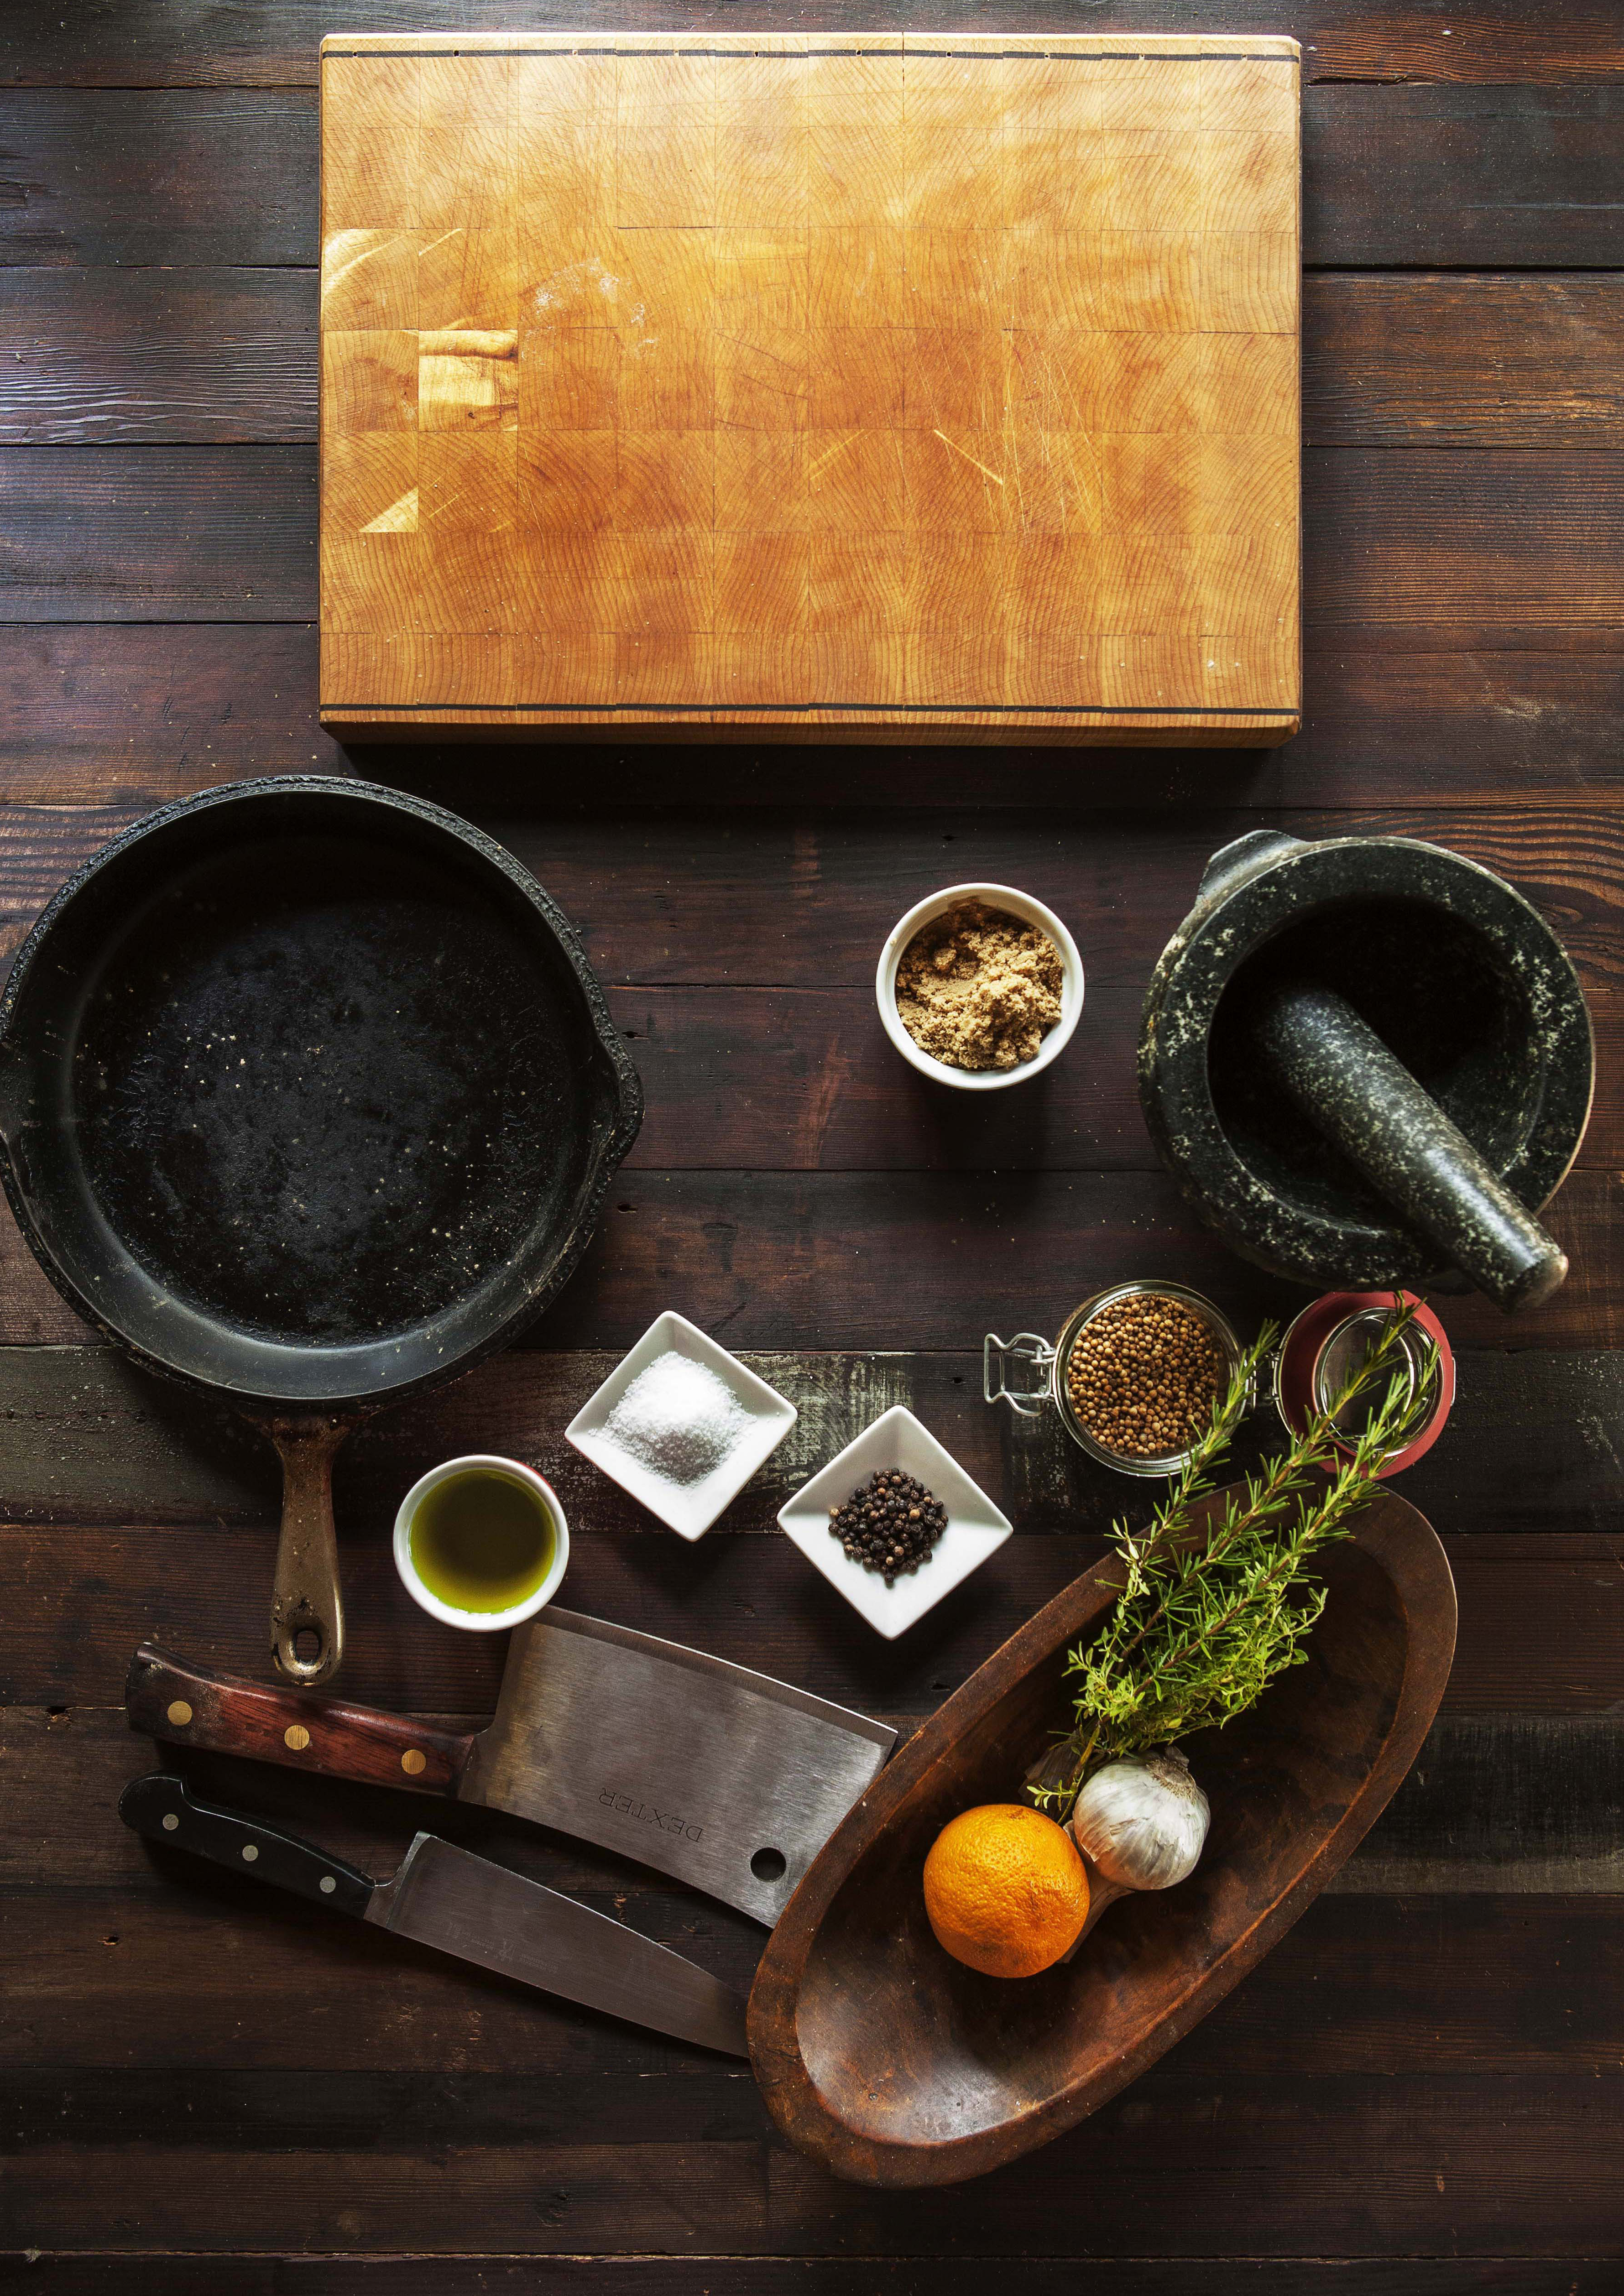
\includegraphics[width=\paperwidth, height=0.45\paperheight]{cover.jpg}
};
\end{tikzpicture}
\begin{minipage}[t][0.5\textheight][t]{\textwidth}
	\vspace*{0.4\paperheight}
	\section*{\sectionformat Nome da Receita}
	\addcontentsline{toc}{section}{Nome da Receita}
	\begin{multicols*}{2}
		\hspace*{-0.28cm}
		\begin{tabu} to 1.04\linewidth {X[l]X[r]}
		   \textit{Serve $3$ pessoas} & \textit{$430$ kcal}
		\end{tabu}\\
		\rule[0.5ex]{\linewidth}{1pt}
		\subsection*{\subsectionformat Teste}
		% \vspace*{-0.8cm}
		\kant[1]
	\end{multicols*}
\end{minipage}
